\documentclass[11pt]{article}
\usepackage{geometry}
\geometry{margin=1.5in}
\usepackage{graphicx}
\usepackage{amssymb}
\usepackage{epstopdf}
\DeclareGraphicsRule{.tif}{png}{.png}{`convert #1 `dirname #1`/`basename #1 .tif`.png}
\usepackage{physics}
\usepackage[dvipsnames]{xcolor}
\usepackage{listings}
\usepackage{hyperref}
\usepackage{multicol}
\usepackage{longtable}
\usepackage{breqn}

%New colors defined below
\definecolor{codegreen}{rgb}{0,0.6,0}
\definecolor{codegray}{rgb}{0.5,0.5,0.5}
\definecolor{codepurple}{rgb}{0.58,0,0.82}
\definecolor{backcolour}{rgb}{0.95,0.95,0.92}

%Code listing style named "mystyle"
\lstdefinestyle{mystyle}{
  backgroundcolor=\color{backcolour},   commentstyle=\color{codegreen},
  keywordstyle=\color{magenta},
  numberstyle=\tiny\color{codegray},
  stringstyle=\color{codepurple},
  basicstyle=\ttfamily\footnotesize,
  breakatwhitespace=false,
  breaklines=true,
  captionpos=b,
  keepspaces=true,
  numbers=left,
  numbersep=5pt,
  showspaces=false,
  showstringspaces=false,
  showtabs=false,
  tabsize=2
}

\lstset{style=mystyle}

\title{DMFortFactor: A FORTRAN Program for Experimental WIMP Analysis}
\author{Oliver Gorton, Changfeng Jiao and Calvin Johnson}

\begin{document}
\maketitle

{

\centering

Model-Independent WIMP Scattering Responses and Event Rates

}

\tableofcontents

This is the manual for the FORTRAN version of the model- independent WIMP 
scattering response and event rate code, which was originally written in 
Mathematica and described in 
\href{http://arxiv.org/abs/1308.6288v1}{arXiv:1308.6288}.

\clearpage

\section{Quickstart guide: Fortran interface}
This program primarily computes two quantities. The first is the WIMP-nucleus
differential event rate spectra:
\begin{dmath}
\frac{dR_D}{dE_R} = \frac{dR_D}{d\vec{q}^2}(q)
	\\= N_T\frac{\rho_\chi}{m_\chi}\int_{v_{min}}^{v_{escape}} 
	\frac{2m_T}{4\pi v^2}\frac{1}{2j_\chi+1}\frac{1}{2j_T+1}
	\sum_{spins}|\mathcal{M}(v,q)|^2  \tilde{f}(\vec{v})vd^3v
\end{dmath}
This quantity has units of events/GeV and is implicitly multiplied by
an effective exposure of 1 Kilogram-Day of target nuclei. This is done by
taking $N_t = 1\ kilogram\cdot day / m_T$, where $m_T$ is the mass of the target
nucleus in $GeV$. Recoil energies $E_R$ are given in keV.

The cross section is determined using a user-defined WIMP-nucleus interaction
within a non-relativistic effective field theory (EFT) framework. The
interaction is specified by 16 coupling coefficients defining an interaction:

\begin{equation}
	\sum_{x=p,n}\sum_{i=1}^{16} c_i^x \mathcal{O}_i
\end{equation}

The second is the integral of the first over either energy or momentum-transfer,
for a range specified by the user. 

\subsection{Required files}
There are two files required for any calculation:
\begin{enumerate}
    \item Control file (.control)
    \item Nuclear density matrix file (.dres)
\end{enumerate}
Additionally, if the user enables the option ``usenergyfile'', then a file
containing the input energies or momentum will also be required.

\subsection{Event rate spectra (events per GeV)}
The program will prompt the user for 
the minimum necessary inputs to run a calculation with default parameter 
values, including the name of a control file which contains the EFT
coefficients, and optionally, additional customizations to the calculation
parameters.

After selecting the option to compute an event rate spectra, there are six
further lines of input. These will be explained by an example:

\begin{verbatim}
 Enter the target proton number
54
 Enter the target neutron number 
77 
 Enter name of control file (.control):
xe131
...
  Enter name of one-body density file (.dres)
xe131gcn
...
 What is the range of recoil energies in kev?
 Enter starting energy, stoping energy, step size:
0.0001 250. 1.0
\end{verbatim}

The first two entries are self-evident: we specifiy the number of protons and
neutrons in the target nucleus. In this case, 54 and 74, respectively, for
$^{131}$Xe.

Third is the name of the control file containing the EFT coefficients and other,
optional, settings. The '.control' file extension is omitted. This contents of
this file will be explained in more detail later.

Fourth is the file containing the nuclear wave functions in the form of one-body
density matrices. Only the ground-state need be included. The '.dres' file
extension is omitted. 

Fifth and finally are three numbers specifying the range of recoil energies
$E_R$ that the differential scattering rate should be computed for.

The event rate spectra will be written to a file, and as a side effect of the
calculation, the total event rate for the energy range requested will be
estimatted by numerical integration. Note that the accuracy of this result will
depend on the choice of the step size.

\subsection{Control file}

Each EFT parameter is written on its own line in [mycontrolfile].control, with
four values: the keyword "coefnonrel", the operator number (integer 1..16), the
coupling type ("p"=proton, "n"=neutron, "s"=scalar, "v"=vecctor), and the
coefficient value. For example, 
\begin{verbatim}
coefnonrel    1    s     3.1
\end{verbatim}
would set $c_1^0 = 3.1$. We take the isospin convention:
\begin{equation}
	\begin{split}
		c^0 = c^p + c^n\\
		c^1 = c^p - c^n
	\end{split}
\end{equation}
Thus, the previous example is equivalent to:
\begin{verbatim}
coefnonrel    1    p     1.55
coefnonrel    1    n     1.55
\end{verbatim}

The control file also serves a more general but optional function: to set any 
parameter in the program to a custom value.  
Simply add an entry to the control file with two values: the first 
should be the keyword for the parameter and the 
second should be the value to set that parameter to. For example, to set the 
velocity of the earth in the galactic frame to $240\ km/s$, you should add the line:
\begin{verbatim}
vearth  240.0
\end{verbatim}

\subsection{Total integrated events}
Inputs 2 - 6 for this calculation will be almost identical to those required for
the event rate spectra calculation. The main difference is in the sixth and
final input:
\begin{verbatim}
 Using adaptive numerical integration to determine total 
 integrated event rate. What are the limits of integration 
 for recoil energies in kev? Enter starting energy, 
 stoping energy, relative error:
0.0 250.0 0.001
\end{verbatim}
Here, we have again been asked for a starting and stopping recoil energy, but
this time the third value is the desired relative error of the integrated
spectra. In this example, 0.001 corresponds to a desired uncertainty of 0.1\%. 

An important difference between this calculation and the event rate spectra
calculation is that in this evaluation, the spectra is not written to file. This
is because an adaptive integration routine is used to keep the number of
function evaluations to a minimum. As a result, this calculation will be much
faster than computing the entire spectra.

\clearpage

\section{Quickstart Guide: Python interface}

We provide two generic API's for interacting with the Fortran program through a
python interface. They are: \textbf{runCustomControl} and
\textbf{runCustomInput}. The former runs the Fortran code with a control file
which has been programatically modified by the API then returns the results to
the calling environment. The latter does the same, except with a custom input
file, rather than a custom control file.

\subsection{Example: using runCustomInput to generate a weighted sum of
event rate spectra}

In this example we will construct a simple python script using the 
runCustomInput API to compute the differential
event rate spectra for several isotopes of Xe, and compute the weighted sum
according to the natural abundances of each isotope.

Firt, examining the API for runCustomInput:

\begin{lstlisting}[language=python]
def runCustomInput(exec_name, input_template, param_dict,
    workdir='', label='runCustom',resultfile='eventrate_spectra.dat'):

    """
     Author: Oliver Gorton, 2020

     This is a function for running an executable program with a custom
     input file by replacing keywords in a template used by the executed
     code.

     exec_name: (string) containing the path to and name of the
         executable you want to run
     input_template: (string) this is an input or control file used by the 
         executable and which will be edited by this function
     param_dict: (dictionary) of keywords and the values to which those 
         keywords will be changed. The keywords are strings which should 
         appear in the input_template file. 
     workdir: (string) name of the working directory where you want to 
         call the executable and send the output.
     label: (string) name for this job, to label the input and output 
         files generated by this function.

    """
\end{lstlisting}
The first three inputs are mandatory while the last three are optional, having
default values defined in the function.
We begin constructing our script by creating the generic inputs for the
executatble name and the directory where the calculations will be done (this is
where the required files for the calculation should be). We also specify the 
atomic number and natural abundances for Xenon isotopes:
\begin{lstlisting}[language=python]
import os
import matplotlib.pyplot as plt
import runCustomInput

exec_name = "dmfortfactor.x"
workdir = os.getcwd()

Z = 54
isotopes = [128, 129, 130, 131, 132, 134, 136]
weights = [.01910, .26401, .04071, .21232, .26909, .10436, .08857]
weightedsum = 0.0
\end{lstlisting}
Now, we will need the input-file template. Having created the template file, for
example:
\begin{verbatim}
1
54
NEUTRONS
xe
xeAAAgcn
1. 1000. 1.0
\end{verbatim}
with our arbitrary choice of keywords "NEUTRONS" and "AAA", 
let's loop over our isotopes, and for each assemble the dictionary of
keywords which the API will replace with values:
\begin{lstlisting}[language=python]
input_template = "input.xeAAA"
for i,isotope in enumerate(isotopes):
    N = isotope - Z
    label = "xe"+str(isotope)
    param_dict = { "NEUTRONS" : N, "AAA" : isotope }
\end{lstlisting}
We now have all of the required arguments: exec\_name, input\_template,
param\_dict, workdir, and label. We are ready to call runCustomInput, which
returns the event rate spectra vs recoil energy arrays. All-together now:
\begin{lstlisting}[language=python]
import os
import matplotlib.pyplot as plt
import runCustomInput

exec_name = "dmfortfactor.x"
workdir = os.getcwd()

Z = 54
isotopes = [128, 129, 130, 131, 132, 134, 136]
weights = [.01910, .26401, .04071, .21232, .26909, .10436, .08857]
weightedsum = 0.0
input_template = "input.xeAAA"
for i,isotope in enumerate(isotopes):
    N = isotope - Z
    label = "xe"+str(isotope)
    param_dict = { "NEUTRONS" : N, "AAA" : isotope }

    RecoilE, EventRate = runCustomInput.runCustomInput(exec_name,
            input_template, param_dict, workdir, label)

    weightedsum += EventRate * weights[i]    
\end{lstlisting}
We now have the weighted sum of event rates stored in the variable weightedsum.
Using matplotlib, we could produce the following plot:

{
	\centering
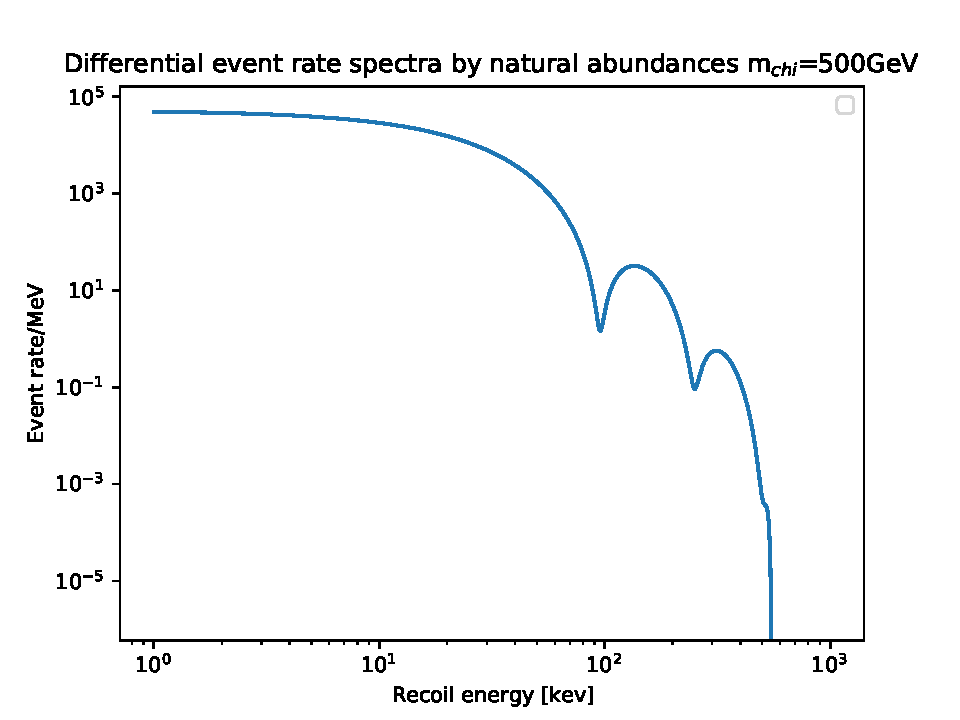
\includegraphics[width=\textwidth]{weightedspectra.pdf}

}

\subsection{Example: using runCustomControl to compare event-rate spectra for
calculations with different WIMP masses}

In this example we will construct a simple python script using the 
runCustomControl API to compute the differential event rate spectra for several
values of the WIMP particle mass. This is very similar in implementation to the
previous example, with the main difference being that the WIMP mass is edited by
the user through the control file, rather than through the interactive input or
input file. The appropriate API for this task is therefore \textbf{
runCustomControl}:
\begin{lstlisting}[language=python]
def runCustomControl(exec_name, inputfile, control_template, param_dict,
    workdir='', label='runCustom',resultfile='eventrate_spectra.dat'):

    """
     Author: Oliver Gorton, 2020

     This is a function for running an executable program with a custom
     control file by replacing keywords in a template used by the executed
     code. The control file is one which is used indirectly (not a by a 
     command line pipe). For example, an interaction file for bigstick.

     exec_name: 
         (string) containing the path to and name of the
         executable you want to run
     inputfile: 
         (string) this is an input file used by the executable
     control_template: 
         (string) the base-name of a file ending in 
         '.control'. "<control_template>.template" is the template 
         file which the function will edit and copy into 
         <control_template>.
     param_dict: 
         (dictionary) of keywords and the values to which those 
         keywords will be changed. The keywords are strings which should 
         appear in the input_template file. 
     workdir: 
         (string) name of the working directory where you want to call
         the executable and send the output.
     label: 
         (string) name for this job, to label the input and output files 
         generated by this function.

    """
\end{lstlisting}
This API has the same inputs as runCustomInput, with `inputfile' intead of
`input\_template', and one additional argument: `control\_template'.

We again start by constructing the necessary arguments:
\begin{lstlisting}[language=python]
import os
import matplotlib.pyplot as plt
import runCustomControl

exec_name = "dmfortfactor.x"
inputfile = 'input.xe131'
control_template = "xe131.control"
workdir = os.getcwd()
\end{lstlisting}
As in the previous example, inputfile is a standard input file we have placed in
the current working directory. This time, it is a complete input file with no
replaceable keywords:
\begin{verbatim}
1
54
77
xe131
xe131gcn
1. 1000. 10.0
\end{verbatim}
Alongside this standard input file, we also create a template control file
called ``xe131.control.template''. When the API replaces the keywords in this
file, it will strip the .template filename extension, creating a file called
``xe131.control'', which is referenced in the fourth line of the above input
file. Within this template file, we find the line (along with other necessary
and/or optional control commands not listed for brevity):
\begin{verbatim}
wimpmass MASS_KEYWORD
\end{verbatim}
`wimpmass' is the keyword for setting the WIMP mass, and `MASS\_KEYWORD' is our
arbitrary keyword for the Python API to replace.

We complete the script by looping over different WIMP masses, creating the
dictionary or keywords to replace and their values, and finally call the
runCustomControl API:
\begin{lstlisting}[language=python]
import os
import matplotlib.pyplot as plt
import runCustomControl

exec_name = "dmfortfactor.x"
inputfile = 'input.xe131'
control_template = "xe131.control"
workdir = os.getcwd()
for wimp_mass in (50.,150.0, 500.,5000.):
    param_dict = { "MASS_KEYWORD" : wimp_mass }
    RecoilE, EventRate = runCustomControl.runCustomControl(exec_name,
            inputfile, control_template, param_dict, workdir)
\end{lstlisting}
We could, for example, plot the result at each iteration and construct the
following plot:

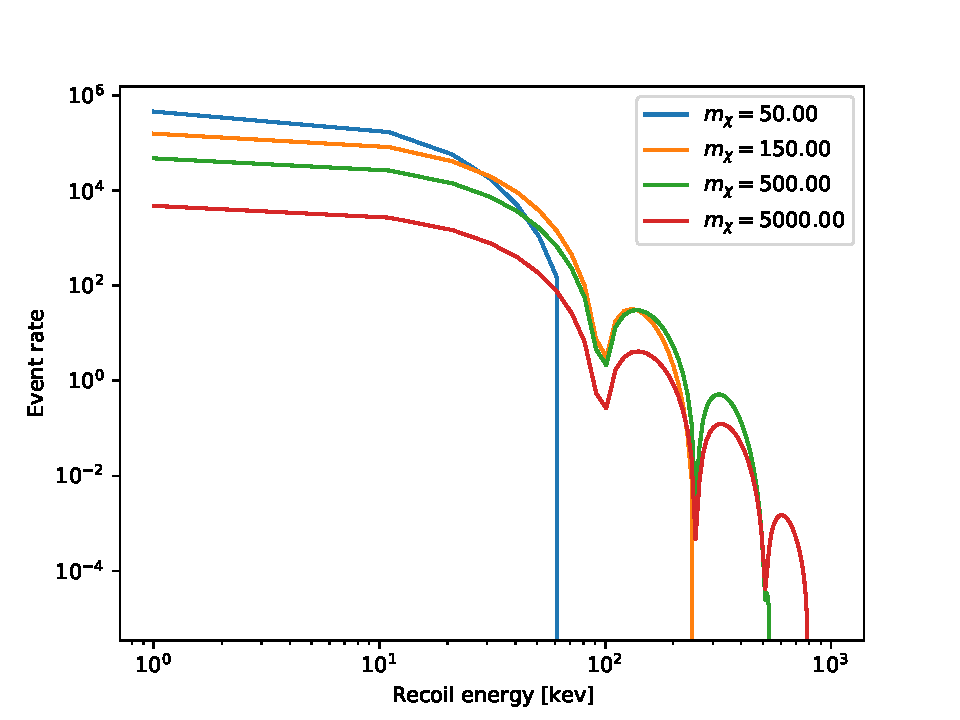
\includegraphics[width=.8 \textwidth]{xe131.WIMPmassCompare.pdf}

\clearpage

\section{Equations found in the code}
\subsection{Differential event rate}
\begin{equation}\label{ER}
\begin{split}
	\frac{dR_D}{dE_R} = \frac{dR_D}{d\vec{q}^2}(q)
	 = N_T n_\chi \int_{v_{min}}^\infty \frac{d\sigma(v,q)}{d\vec{q}^2} \tilde{f}(\vec{v})vd^3v
\end{split}
\end{equation}
where $q$ is the WIMP-nucleon momentum transfer, $N_T$ is the number of target 
nuclei, $n_\chi = \rho_\chi/m_\chi$ is the local dark matter number density, $\sigma$ 
is the WIMP-nucleon cross section, and $\tilde{f}$ is dark matter velocity 
distribution in the lab-frame. $\tilde{f}(\vec{v})$ is obtained by boosting 
the Galactic-frame distribution $f(\vec{v})$, 

\begin{equation}\label{boost}
\begin{split}
	\tilde{f}(\vec{v}) = f(\vec{v} + \vec{v}_{earth}),
\end{split}
\end{equation}
where $\vec{v}_{earth}$ is the velocity of the earth in the galactic rest 
frame. The simplest model is a three-dimensional Maxwell distribution:

\begin{equation}
\begin{split}
	f(\vec{v}) \propto e^{-\vec{v}^2/v_0^2},
\end{split}
\end{equation}
where $v_0$ is some scaling factor (typically taken to be around $220\ km/s$).

In order to evaluate the integral in (\ref{ER}), we make the conversion to 
spherical coordinates, and take special care to deal with the velocity boost 
in (\ref{boost}). Assuming a $1/v^2$ velocity dependence of the cross section 
term (see section \ref{crosssection}), we need to evaluate an integral of the 
form
\begin{equation}
\begin{split}
	I = \int_{v_{min}}^{v_{max}} d^3v \frac{f(\vec{v} + \vec{v}_{earth})}{v} =
    	\int_{v_{min}}^{v_{max}} d^3v \frac{1}{v} e^{-(\vec{v}+\vec{v}_{earth})^2/v_0^2}
\end{split}
\end{equation}
Noting that $(\vec{v}+\vec{v}_{earth})^2 = \vec{v}^2 + \vec{v}^2_{earth} + 
2vv_{earth}\cos(\theta)$, with $|\vec{v}|\equiv v$ and $\theta$ defining 
the angle between the two vectors, it's convenient to make the substitution 
$d^3v = d\phi d(\cos \theta) v^2 dv$:
\begin{equation}
\begin{split}
	I &=  \int_0^{2\pi} d\phi \int_{v_{min}}^{v_{max}} dv \int_{-1}^1 d(\cos \theta) e^{-2vv_{earth}\cos\theta/v_0^2} v^2 \frac{1}{v} e^{-(\vec{v}^2+\vec{v}^2_{earth})/v_0^2}\\
	&= 2\pi \int_{v_{min}}^{v_{max}} dv v e^{-(\vec{v}^2+\vec{v}^2_{earth})/v_0^2} \left(-\frac{v_0^2}{2vv_{earth}} e^{-2vv_{earth}\cos\theta/v_0^2}\right)_{-1}^1\\
	&= \frac{\pi v_0^2}{v_{earth} }\int_{v_{min}}^{v_{max}} dv e^{-(\vec{v}^2+\vec{v}^2_{earth})/v_0^2} 
		\left(- e^{-2vv_{earth}/v_0^2} + e^{+2vv_{earth}/v_0^2}\right)\\
	&= \frac{\pi v_0^2}{v_{earth} }\int_{v_{min}}^{v_{max}} dv 
		\left(- e^{(v+v_{earth})^2/v_0^2} + e^{(v-v_{earth})^2/v_0^2}\right)\\
	&= \frac{\pi v_0^2}{v_{earth} }\int_{v_{min}}^{v_{max}} dv 
		\left( g(v-v_{earth}) - g(v+v_{earth}) \right)
\end{split}
\end{equation}
where in the last equality, we have defined a one-dimensional Gaussian form
\begin{equation}
\begin{split}
	g(v) \propto e^{-v^2/v_0^2}.
\end{split}
\end{equation}

The final expression for $I$ can be trivially generalized to other spherically
symmetric velocity-dependent forms of the differential cross section. What's 
important is the reduction of the velocity-boosted $d^3v$ integral to a radial 
integral which can be carried out with one-dimensional quadrature:
\begin{equation}\label{integral}
\begin{split}
\int_{v_{min}}^{v_{max}} d^3v \sigma(v) e^{-(\vec{v}+\vec{v}_{earth})^2/v_0^2}
\\
	= \frac{\pi v_0^2}{v_{earth} }\int_{v_{min}}^{v_{max}} dv \sigma(v) v^2\left( g(v-v_{earth}) - g(v+v_{earth}) \right).
\end{split}
\end{equation}
The FORTRAN code uses equation (\ref{integral}) to evaluate the event rate 
integral in equation (\ref{ER}) with quadrature. Analytic solutions of  
(\ref{integral}) exist in the form of error functions; we use the above form 
since it makes easy to later modify the velocity distribution (as long as it 
remains spherically symmetric). For example, adding a velocity cut-off is as 
easy as changing the limit on the quadrature, with no need to write a whole 
new subroutine for the analytic forms found in the Mathematica script.

\subsection{Differential cross section}\label{crosssection}
\begin{equation}
\begin{split}
\frac{d\sigma(v,E_R)}{dE_R} = 2m_T \frac{d\sigma(v)(v,\vec{q}^2)}{d\vec{q}^2} = 2m_T\frac{1}{4\pi v^2}T(v,q),
\end{split}
\end{equation}
Where $v$ is the velocity of the dark matter particles in the lab-frame, $q$ is the momentum transfer of the scattering event, $m_T$ is the mass of the target nucleus, and $T(v,q)$ is the transition or scattering probability. We can see here that the differential cross section has an explicit $1/v^2$ dependence, independent of any velocity dependence of $T(v,q)$.


\subsection{Transition probability / Scattering probability}

The scattering probability is

\begin{equation}
\begin{split}
T(v,q) &= \frac{1}{2j_\chi+1}\frac{1}{2j_T+1}\sum_{spins}|\mathcal{M}(v,q)|^2 
\end{split}
\end{equation}
where $j_\chi$ is the spin of the WIMP, $j_T$ is the spin angular momentum of the target nucleus, and $\mathcal{M}$ Galilean invariant amplitude, which is defined by
\begin{align}
	T(v,q) = \frac{4\pi}{2j_T+1}\frac{1}{(4m_\chi)^2}
		\sum_{x=p,n}\sum_{x'=p,n}^1\sum_{i=1}^8 R_i^{xx'}(v^2,q^2)
		W_i^{xx'}(q)
%		\left < \mathcal{O}_{j_T,x}^{(i)}(y)\right >
%		\left < \mathcal{O'}_{j_T,x'}^{(i)}(y)\right >
\end{align}
where $m_\chi$ is the mass of the dark matter particle and $x$ is an index used to sum over isospin couplings. The coefficients $R_i^{x,x'}$ are dark matter particle response functions, to be define in another section. The operators $W_i^{xx'}(q)$ are nuclear response functions, which are sums over matrix elements of nuclear operators constructed from Bessel spherical harmonics and vector spherical harmonics.
\subsection{Dark matter response functions}
There are 8 dark matter response functions which group 15 operator coefficients $c_i^x$ according the pair of nuclear response functions which they multiply.

%%%%%%%%%%%%%%%%%%%%%%%%%%%%%%%%%%%%%%%%%%%%%%%%%%%%%%%%%%%%%%%%%%%%%%%%%%%%%%80
% Tex formatting style for this section: 
%   * parenthesis hierarchy: \{, [, (
%   * zero indent for new definition or equality
%   * single indent for new print line (usage of \\)
%   * double indent for source line continuation without new print line
\begin{dmath}
R_{M}^{xx'}(v,q) = \frac{1}{4}cl(j_\chi) \{ [v^2-(q/2\mu_t)^2] 
        (c_5^{x}c_5^{x'}q^2 + c_8^{x}c_8^{x'}) + c_{11}^{x}c_{11}^{x'}q^2 \}
    + \{c_1^{x} + c_2^{x}[v^2-(q/2\mu_t)^2] \} \{c_1^{x'} 
        + c_2^{x'}[v^2-(q/2\mu_t)^2] \} 
\end{dmath}
%%%%%%%%%%%%%%%%%%%%%%%%%%%%%%%%%%%%%%%%%%%%%%%%%%%%%%%%%%%%%%%%%%%%%%%%%%%%%%80
\begin{dmath}
R_{\Sigma''}^{xx'}(v,q) = \frac{1}{16}cl(j_\chi) \{c_6^{x}c_6^{x'}q^4 
    + (c_{13}^{x}c_{13}^{x'}q^2 + c_{12}^{x} c_{12}^{x'} ) [v^2 
    - (q/2\mu_T)^2 ] + 2c_4^xc_6^{x'}q^2 + c_4^xc_4^{x'}\} 
    + \frac{1}{4}c_{10}^xc_{10}^{x '}q^2
\end{dmath}
%%%%%%%%%%%%%%%%%%%%%%%%%%%%%%%%%%%%%%%%%%%%%%%%%%%%%%%%%%%%%%%%%%%%%%%%%%%%%%80
\begin{dmath}
R_{\Sigma'}^{xx'}(v,q) = \frac{1}{32} cl(j_\chi) \{ 2c_{9}^{x}c_{9}^{x'}q^2 
        + ( c_{15}^{x}c_{15}^{x'}q^4 + c_{14}^{x}c_{14}^{x'}q^2 
        - 2c_{12}^{x}c_{15}^{x'} q^2 + c_{12}^{x}c_{12}^{x'}) [v^2-(q/2\mu_T)^2]
        + 2c_{4}^{x}c_{4}^{x'} \} 
        +\frac{1}{8}(c_{3}^{x}c_3^{x'}q^2 + c_{7}^{x}c_{7}^{x'})[v^2-(q/2\mu_T)^2]
\end{dmath}
%%%%%%%%%%%%%%%%%%%%%%%%%%%%%%%%%%%%%%%%%%%%%%%%%%%%%%%%%%%%%%%%%%%%%%%%%%%%%%80
\begin{dmath}
R_{\Phi''}^{xx'}(v,q) = \frac{q^2}{(4m_N)^2}cl(j_\chi) (c_{12}^x - c_{15}^{x}q^2
        )(c_{12}^{x '}-c_{15}^{x '}q^2 ) 
    + \frac{q^2}{(4m_N)^2}q^2c_3^x c_3^{x'} 
\end{dmath}
%%%%%%%%%%%%%%%%%%%%%%%%%%%%%%%%%%%%%%%%%%%%%%%%%%%%%%%%%%%%%%%%%%%%%%%%%%%%%%80
\begin{dmath}
R_{\tilde{\Phi}'}^{xx'}(v,q) = \frac{q^2}{(4m_N)^2}cl(j_\chi)(
        c_{12}^xc_{12}^{x'}q^2 + c_{12}^x c_{12}^{x'})
\end{dmath}
%%%%%%%%%%%%%%%%%%%%%%%%%%%%%%%%%%%%%%%%%%%%%%%%%%%%%%%%%%%%%%%%%%%%%%%%%%%%%%80
\begin{dmath}
R_{\Delta}^{xx'}(v,q) = \frac{q^2}{(2m_N)^2}cl(j_\chi) (c_{5}^{x}c_{5}^{x'}q^2 
        + c_{8}^{x}c_{8}^{x'}) 
        + 2\frac{q^2}{m_N^2}c_{2}^{x}c_{2}^{x'}[v^2-(q/2\mu_T)^2]
\end{dmath}
%%%%%%%%%%%%%%%%%%%%%%%%%%%%%%%%%%%%%%%%%%%%%%%%%%%%%%%%%%%%%%%%%%%%%%%%%%%%%%80
\begin{dmath}
R_{\Delta \Sigma'}^{xx'}(v,q) = \frac{q^2}{(2m_N)^2}cl(j_\chi) 
        (c_{4}^{x}c_{5}^{x'} - c_{8}^{x}c_{9}^{x'}) 
        - \frac{q^2}{m_N} c_{2}^{x}c_{3}^{x'} [v^2-(q/2\mu_T)^2]
\end{dmath}
%%%%%%%%%%%%%%%%%%%%%%%%%%%%%%%%%%%%%%%%%%%%%%%%%%%%%%%%%%%%%%%%%%%%%%%%%%%%%%80
\begin{dmath}
R_{\Phi''M}^{xx'}(v,q) = \frac{q^2}{4m_N}cl(j_\chi)c_{11}^{x}
        (c_{12}^{x'} - c_{15}^{x'} q^2) 
        + \frac{q^2}{m_N}c_{3}^{x'}  \{c_{1}^{x} + c_{2}^{x} [v^2-(q/2\mu_T)^2]\}
\end{dmath}
%%%%%%%%%%%%%%%%%%%%%%%%%%%%%%%%%%%%%%%%%%%%%%%%%%%%%%%%%%%%%%%%%%%%%%%%%%%%%%80
As a shorthand we have introduced the notation 
\begin{align}
	cl(j) = 4j(j+1)/3.
\end{align}


\subsection{Nuclear response functions}
There are eight nuclear response functions $W_i^{xx'}(y)$ considered 
here. The unit-less variable $y$ is defined 
\begin{align}
 y = \left ( \frac{qb}{2} \right) ^2,
 \end{align}
 in terms of the harmonic oscillator size parameter $b$, which has a default value of 
 \begin{align}
b^2 = 41.467/(45A^{-1./3} - 25A^{-2/3})\ fm^2.
 \end{align}

 
\begin{align}
W_M^{xx'}(y) &= \sum_{even\ J} 
\bra{j_T}M_{Jx}(y)\ket{j_T}
\bra{j_T}M_{Jx'}(y)\ket{j_T}
\\
W_{\Sigma''}^{xx'}(y) &= \sum_{odd\ J} 
\bra{j_T}{\Sigma''}_{Jx}(y)\ket{j_T}
\bra{j_T}{\Sigma''}_{Jx'}(y)\ket{j_T}
\\
W_{\Sigma'}^{xx'}(y) &= \sum_{odd\ J} 
\bra{j_T}{\Sigma'}_{Jx}(y)\ket{j_T}
\bra{j_T}{\Sigma'}_{Jx'}(y)\ket{j_T}
\\
W_{\Phi''}^{xx'}(y) &= \sum_{even\ J} 
\bra{j_T}{\Phi''}_{Jx}(y)\ket{j_T}
\bra{j_T}{\Phi''}_{Jx'}(y)\ket{j_T}
\\
W_{\tilde{\Phi}'}^{xx'}(y) &= \sum_{even\ J} 
\bra{j_T}{\tilde{\Phi}'}_{Jx}(y)\ket{j_T}
\bra{j_T}{\tilde{\Phi}'}_{Jx'}(y)\ket{j_T}
\\
W_{\Delta}^{xx'}(y) &= \sum_{odd\ J} 
\bra{j_T}{\Delta}_{Jx}(y)\ket{j_T}
\bra{j_T}{\Delta}_{Jx'}(y)\ket{j_T}
\\
W_{\Delta\Sigma'}^{xx'}(y) &= \sum_{odd\ J} 
\bra{j_T}{\Delta}_{Jx}(y)\ket{j_T}
\bra{j_T}{\Sigma'}_{Jx'}(y)\ket{j_T}
\\
W_{\Phi''M}^{xx'}(y) &= \sum_{even\ J} 
\bra{j_T}{\Phi''}_{Jx}(y)\ket{j_T}
\bra{j_T}{M}_{Jx'}(y)\ket{j_T}
\end{align}


\subsection{Nuclear operators and their matrix elements}
of which there are six, are nuclear operators constructed from Bessel 
spherical harmonics and vector spherical harmonics, and are evaluated here on 
the ground state of the target nucleus.

\section{Control file keywords}

\begin{longtable}{| l | c | p{2.5in} | c | l | }
  \hline Keyword & Symbol & Meaning & Units & Default \\

  \hline dmdens & $\rho_\chi$ & Local dark matter density. & GeV/cm$^3$ & 0.3\\

  \hline dmspin & $j_\chi$ & Instrinsic spin of WIMP particles. & $\hbar$ &
  $\frac{1}{2}$ \\

  \hline fillnuclearcore & & Logical flag (enter 0 for False, 1 for True) to fill the
  inert-core single-particle orbitals in the nuclear level densities.
  Phenomenological shell model calculations typically provide only the density
  matrices for the active valence-space orbitals, leaving it to the user to
  infer the core-orbital densities. This option automatically assigns these
  empty matrix elements assuming a totally filled core. & & 1 (true)\\
  
  \hline gaussorder & n & Order of the Gauss-Legendre quadrature to use when using Type 2 quadrature. (See quadtype.) An n-th order routine will perform n function evaluations.  Naturally, a higher order will result in higher precision, but longer compute time. & & 12\\

  \hline hofrequency & $\hbar \omega$ & Set the harmonic oscillator length by
  specifying the harmonic oscillator frequency. (b = 6.43/sqrt($\hbar\omega$)).
  If using an \textit{ab initio} interaction, $\hbar \omega$ should be set to
  match the value used in the interaction.
              & MeV & See hoparameter.\\

  \hline hoparameter & $b$ & Harmonic oscillator length. Determines the scale of the
  nuclear wavefunction interaction. & fm &
  $(\frac{41.467}{45A^{-1/3}-25A^{-2/3}})^{1/2}$  \\

  \hline maxwellv0 & $v_0$ & Maxwell-Boltzman velocity distribution scaling factor. &
  km/s & 220.0 \\

  \hline mnucleon & $m_N$ & Mass of a nucleon. It's assumed that $m_p\approx m_n$. &
  GeV & 0.938272 \\

  \hline ntscale & $N_t$ & Effective number of target nuclei scaling factor. The
  differential event rate is multiplied by this constant in units of
  kilogram-days. For example, if the detector had a total effective exposure of
  2500 kg days, one might enter 2500 for this value. & kg days & 1.0 \\
  
  \hline quadrelerr &  & Desired relative error for the adaptive numerical quadrature routine (quadtype 1).  & & $10^{-6}$\\
  
  \hline quadtype & & Option for type of numerical quadrature. (Type 1 = adaptive 8th order Gauss-Legendre quadrature.  Type 2 = static n-th order Gauss-Legendre quadrature.) && 1 (type 1)\\

  \hline useenergyfile & & Logical flag (enter 0 for False, 1 for True) to read energy
  grid used for calculation from a user-provided file intead of specifying a
  range. & & 0 (false) \\

  \hline usemomentum & & Logical flag (enter 0 for False, 1 for True) to use momentum
  transfer intead of recoil energy as the independent variable. & &0 (false) \\

  \hline vearth & $v_{earth}$ & Speed of the earth in the galactic frame. & km/s & 
  232.0\\

  \hline vescape & $v_{escape}$ & Galactic escape velocity. Particles moving faster than
  this speed will escape the galaxy, thus setting an upper limit on the WIMP
  velocity distribution. & km/s & 12 $\times\ v_{scale}$ \\

  \hline weakmscale & $m_v$ & Weak interaction mass scale. User defined EFT coefficients
  are divided by $m_v^2$. & GeV & 246.2 \\

  \hline wimpmass & $m_\chi$ & WIMP particle mass. & GeV & 50.0\\
  \hline
\end{longtable}

\end{document}
